% =====================================================================
%  IoT-IDS conference paper -- IEEE conference format (IEEEtran)
%  Build:  cd paper && latexmk -pdf main.tex      (or: pdflatex, bibtex,
%          pdflatex, pdflatex).  Data: python paper/make_data.py
%  Red [TBD: ...] markers are values that do not exist yet. Set \finaltrue
%  below before submission: the build then FAILS if any marker is left.
% =====================================================================
\documentclass[conference]{IEEEtran}
\IEEEoverridecommandlockouts

\usepackage{cite}
\usepackage{amsmath,amssymb}
\usepackage{graphicx}
\usepackage{textcomp}
\usepackage{xcolor}
\usepackage{booktabs}
\usepackage{multirow}
\usepackage{url}
\usepackage[binary-units]{siunitx}
\usepackage{tikz}
\usetikzlibrary{arrows.meta,positioning}
\usepackage{pgfplots}
\usepgfplotslibrary{groupplots}
\pgfplotsset{compat=1.16}

\newif\iffinal
\finalfalse   % set \finaltrue for the submission build
\newcommand{\TBD}[1]{\iffinal\errmessage{Unresolved TBD: #1}\else
  \textcolor{red}{[TBD: #1]}\fi}

\def\BibTeX{{\rm B\kern-.05em{\sc i\kern-.025em b}\kern-.08em
    T\kern-.1667em\lower.7ex\hbox{E}\kern-.125emX}}

\begin{document}

\title{From Synthetic Benchmarks to a Live Network:\\
Deploying and Auditing a Lightweight Flow-Based\\
IoT Intrusion Detector on a Raspberry Pi~2}

% Author order and e-mail addresses must be confirmed by the team.
\author{
\IEEEauthorblockN{Mahi Patel}
\IEEEauthorblockA{\textit{Dept. of Computer Engineering}\\
\textit{COEP Technological University}\\
Pune, India\\
\TBD{e-mail}}
\and
\IEEEauthorblockN{Malhar Falke}
\IEEEauthorblockA{\textit{Dept. of Computer Engineering}\\
\textit{COEP Technological University}\\
Pune, India\\
\TBD{e-mail}}
\and
\IEEEauthorblockN{Yugandhar Pise}
\IEEEauthorblockA{\textit{Dept. of Computer Engineering}\\
\textit{COEP Technological University}\\
Pune, India\\
\TBD{e-mail}}
\and
\IEEEauthorblockN{Vaibhav Tayade}
\IEEEauthorblockA{\textit{Dept. of Computer Engineering}\\
\textit{COEP Technological University}\\
Pune, India\\
\TBD{e-mail}}
\and
\IEEEauthorblockN{S. K. Gaikwad}
\IEEEauthorblockA{\textit{Dept. of Computer Engineering}\\
\textit{COEP Technological University}\\
Pune, India\\
\TBD{e-mail}}
}

\maketitle

% ---------------------------------------------------------------------
\begin{abstract}
Machine-learning intrusion detectors for Internet of Things (IoT) networks
are usually reported with near-perfect accuracy on benchmark data, yet few
are measured after deployment on the constrained hardware they target. We
built a complete flow-based detector and followed it from a synthetic
benchmark onto a live network. A single 22-feature extractor serves both
training and detection, and a 92~KB gradient-boosted tree model classifies
ten traffic classes. Because no 32-bit ARM build of the usual inference
runtime exists, we compiled the model to dependency-free C and ran it on a
Raspberry Pi~2, where it reproduced the reference labels on 5{,}000 inputs.
On synthetic held-out traffic the model scored 99.65\% accuracy, but
removing features and changing the split did not move this score, which
shows that the generated classes are trivially separable rather than that
the detector is accurate. On the Raspberry Pi~2, all seven controlled
attacks raised an incident within 21~s, and the sensor ran for 14.4~h with
no restart and no interface packet loss. Ordinary home-network traffic,
however, produced 1.9--2.6 false-alarm incidents per minute, and confidence
thresholds did not remove them. A post-hoc incident-size rule removed every
benign incident but also two of the seven attacks. We further report a
leakage error found in our own earlier cross-dataset study and the
corrected protocol. The results argue that edge intrusion detectors should
be evaluated on representative benign traffic before any accuracy figure is
reported.
\end{abstract}

\begin{IEEEkeywords}
Internet of Things, intrusion detection, edge computing, Raspberry Pi,
gradient boosting, false alarms, evaluation methodology
\end{IEEEkeywords}

% ---------------------------------------------------------------------
\section{Introduction}

IoT devices are attractive targets because they are numerous, rarely
patched, and often reachable with default credentials; the Mirai botnet
showed how quickly such devices can be recruited at scale
\cite{antonakakis2017mirai}. Network intrusion detection is a natural
defence, and machine learning (ML) has become its dominant research
approach \cite{zarpelao2017survey,hajiheidari2019ids,khraisat2021critical}.
Published detectors routinely report accuracy above 99\% on public
datasets. Two gaps remain between these figures and a working sensor.

First, the hardware gap. A detector intended for an IoT gateway must run
on a few hundred megabytes of memory and a low-power CPU, often without the
runtimes used during development. Many studies measure inference speed on a
workstation and leave deployment as future work.

Second, the evaluation gap. Security ML is prone to pitfalls such as
sampling bias, data leakage between training and test data, and lab-only
evaluation \cite{sommer2010outside,arp2022dos,apruzzese2023sok}. Public
intrusion datasets also contain labelling and construction artefacts
\cite{engelen2021troubleshooting,kenyon2020datasets}. A model can then
score highly by learning how a dataset was made rather than what an attack
looks like. Benign traffic is the critical case: a sensor sees benign
traffic almost all the time, so even a small false-positive rate per flow
produces a stream of alerts.

This paper follows one lightweight detector across both gaps. Our
contributions are:
\begin{enumerate}
\item An end-to-end, open flow-based IoT detector in which one packet-to-flow
feature extractor serves both training and live detection, and a compact
tree model is exported to dependency-free C. We show that the C model
reproduces the reference labels exactly on a 32-bit Raspberry Pi~2.
\item A deployment measurement on that board: inference latency, packet
parsing throughput, capture loss under floods, memory, temperature, reboot
recovery, and a 14.4-hour soak.
\item An evaluation audit. We show that a near-perfect synthetic score is
uninformative, and measure what happens on a live home network: controlled
attacks are detected, but benign traffic triggers a sustained false-alarm
rate that confidence thresholds do not remove. We quantify the trade-off of
a simple incident-size filter.
\item A corrected cross-dataset protocol over eleven public datasets,
including a report of the resubstitution error that invalidated our own
earlier result.
\end{enumerate}

Section~\ref{sec:related} reviews related work. Section~\ref{sec:system}
describes the system and Section~\ref{sec:method} the evaluation method.
Section~\ref{sec:results} presents the results, Section~\ref{sec:discussion}
discusses their implications and limitations, and Section~\ref{sec:conclusion}
concludes.

% ---------------------------------------------------------------------
\section{Related Work}\label{sec:related}

\textit{IoT intrusion detection.}
Surveys group IoT detectors by placement, detection method and validation
strategy, and note that most proposals are validated by simulation or on
offline datasets rather than in deployment
\cite{zarpelao2017survey,hajiheidari2019ids,khraisat2021critical}.
Lightweight online detectors exist: Kitsune trains an ensemble of small
autoencoders on per-packet statistics and runs on a Raspberry Pi
\cite{mirsky2018kitsune}, and N-BaIoT detects botnet traffic per device
with deep autoencoders \cite{meidan2018nbaiot}. Our work differs in that it
uses a supervised multiclass flow model, exports it to plain C, and measures
benign false alarms on a live network.

\textit{Evaluation pitfalls.}
Sommer and Paxson argued that intrusion detection differs from other ML
tasks because errors are costly and benign traffic is highly diverse
\cite{sommer2010outside}. Arp \textit{et al.} catalogued pitfalls including
data snooping, spurious correlations and lab-only evaluation
\cite{arp2022dos}, and Apruzzese \textit{et al.} call for assessments that
reflect operational constraints \cite{apruzzese2023sok}. Leakage, where
information about the test data reaches training, is a general cause of
over-optimistic results \cite{kaufman2012leakage}. We encountered both
spurious separability and leakage in our own pipeline and report them.

\textit{Cross-dataset generalisation.}
Flow datasets use different feature extractors, such as CICFlowMeter
\cite{lashkari2017cicflowmeter} or Zeek, which complicates comparison.
Sarhan \textit{et al.} proposed a standard NetFlow-based feature set so
that detectors can be compared across datasets \cite{sarhan2022standard}.
Our cross-dataset study instead aligns eleven datasets' native features
into a common twelve-feature space by meaning and unit
(Section~\ref{sec:sfaf}).

% ---------------------------------------------------------------------
\section{System Design}\label{sec:system}

\begin{figure}[t]
\centering
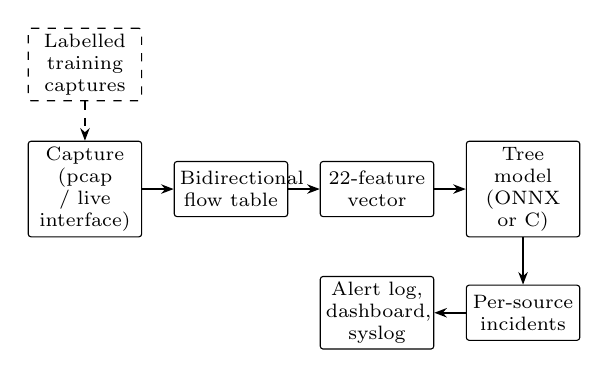
\begin{tikzpicture}[
  node distance=3mm and 4mm,
  box/.style={draw, rounded corners=1pt, align=center, font=\scriptsize,
              minimum height=7mm, inner sep=2pt, text width=13mm},
  arr/.style={-{Stealth[length=1.6mm]}, semithick}]
\node[box] (cap) {Capture\\(pcap / live\\interface)};
\node[box, right=of cap] (flow) {Bidirectional\\flow table};
\node[box, right=of flow] (feat) {22-feature\\vector};
\node[box, right=of feat] (model) {Tree model\\(ONNX or C)};
\node[box, below=6mm of model] (inc) {Per-source\\incidents};
\node[box, left=of inc] (out) {Alert log,\\dashboard,\\syslog};
\node[box, above=5mm of cap, dashed] (train)
     {Labelled\\training\\captures};
\draw[arr] (cap) -- (flow);
\draw[arr] (flow) -- (feat);
\draw[arr] (feat) -- (model);
\draw[arr] (model) -- (inc);
\draw[arr] (inc) -- (out);
\draw[arr, dashed] (train) -- (cap);
\end{tikzpicture}
\caption{Detection pipeline. Training captures (dashed) pass through the
same capture-to-feature path as live traffic, so there is no separate
training-time feature code.}
\label{fig:arch}
\end{figure}

\subsection{Flow features}
The pipeline is shown in Fig.~\ref{fig:arch}. Packets are parsed from a
capture file or a live interface (Ethernet, VLAN, IPv4, IPv6, TCP, UDP and
ICMP) and grouped into bidirectional flows keyed by protocol and endpoints.
Each flow is summarised by 22 features: protocol, duration, packet and byte
counts in each direction, packet and byte rates, packet-length and
inter-arrival statistics, TCP SYN/FIN/RST/ACK ratios, direction asymmetry,
the destination service port, and three \emph{host-context} features that
count the distinct destination ports and hosts contacted by the source in
a rolling window. Host context separates attacks that look identical at
the level of a single flow: a port scan touches many ports on one host, a
Mirai-style propagation touches one port on many hosts, and a flood sends
heavy traffic to one host and port. The feature layout is versioned, and
the detector refuses a model built for a different layout.

\subsection{Model and export}
The classifier is an XGBoost multiclass model \cite{chen2016xgboost} over
ten classes: benign, three reconnaissance or brute-force classes (port scan,
Xmas/NULL/FIN scan, SSH brute force), five denial-of-service classes (SYN,
UDP, ICMP and MQTT floods, and slowloris) and a Mirai-style botnet class.
It has 1{,}200 trees with 2{,}780 nodes in total. Trees are invariant to
feature scaling, so no scaler is shipped. The model is exported to ONNX
(91.8~KB) for ONNX Runtime \cite{onnxruntime} and, by our own exporter, to
a single C99 header containing about 49~KB of constant node data. The C
inference function uses no heap and about 130~bytes of stack. The exporter
verifies that the C model makes the same decisions as the XGBoost model.

\subsection{Incidents}
Per-flow verdicts are aggregated into incidents keyed by source address and
attack type, so a 700-port scan produces one incident rather than 700
alerts. An incident is reported when a flow of that type exceeds a
confidence threshold (0.5 by default). Incidents are written to a log, a
local web dashboard, and optionally a syslog collector. An experimental
response module can rate-limit or block a source, but it is disabled in
all results below except one experiment in Section~\ref{sec:discussion}.

% ---------------------------------------------------------------------
\section{Evaluation Method}\label{sec:method}

\subsection{Synthetic training corpus}
Labelled IoT packet captures with a ground truth that can be joined to our
own flow extractor were not available to us. We therefore generated
traffic with Scapy \cite{scapy}: each scenario mixes benign background
traffic with one attack, and a ``hard benign'' family produces bursty
transfers and multi-host telemetry that resemble attacks. The corpus has
350 scenarios. We split it \emph{by scenario} (280 for training and 70 for
testing) so that no attacker, address set or timing pattern appears on
both sides; this gives 44{,}761 training flows and 12{,}191 test flows.
Two further synthetic sets were generated from unseen random seeds for
validation and benchmarking. We report all three separately.

\subsection{Deployment board and live network}
The deployment board is a Raspberry Pi~2 Model~B (BCM2836, four Cortex-A7
cores, 1~GB RAM) running 32-bit Raspberry Pi OS (Debian~13, Python~3.13).
ONNX Runtime publishes no wheels for 32-bit ARM, so the board runs the C
model through a thin \texttt{ctypes} wrapper. To check that this changes
nothing, we also built ONNX Runtime 1.23.2 for armv7 from source.
The sensor was installed as a system service with its default settings.
The live trial used an ordinary home network (\texttt{/24} IPv4 subnet with
IPv6) and devices owned by the authors only.

\subsection{Live experiments}
\begin{itemize}
\item \textit{Controlled attacks.} Seven attacks were run one at a time
with standard tools: a TCP connect scan and an Xmas scan (\texttt{nmap}),
SYN, UDP and ICMP floods at about 2{,}000 packets/s for 20~s
(\texttt{hping3}), 40 failed SSH logins, and slowloris with 40 held
connections. Network attacks came from a laptop on the same network. The
floods and the Xmas scan were run from the Pi against itself on the
loopback interface so that no flood left the board.
\item \textit{Benign baselines.} Two ten-minute windows with no attacks:
the first observed live, the second captured with \texttt{tcpdump}
(headers only) and replayed through the same detector so that distinct
flows could be counted.
\item \textit{Soak.} The service was sampled every five minutes for
14.4~h (service state, restarts, memory, temperature, throttling,
interface drops, packet and incident counters).
\item \textit{Reboot.} Time from a reboot command to a fresh sensor
heartbeat.
\end{itemize}

\subsection{Cross-dataset protocol}\label{sec:sfaf}
For the research track we aligned eleven public flow datasets
\cite{sharafaldin2018cicids2017,moustafa2015unswnb15,alsaedi2020toniot,
koroniotis2019botiot,neto2023ciciot2023,sharafaldin2019cicddos2019,
ullah2020iotid20,alhawawreh2022xiiotid,hindy2021mqtt,zolanvari2021wustl,
garcia2020iot23}
into twelve shared features by meaning and unit: durations are converted to
seconds, missing rates are derived from counts and duration where possible,
and a feature a dataset cannot provide is left missing rather than filled
with zero, because a constant column would reveal the dataset's identity.
For each dataset a binary model is trained on a fixed stratified 80\% split.
The diagonal of the resulting $11\times 11$ matrix is measured on the
untouched 20\%; every off-diagonal cell tests on a different dataset. We
report ROC-AUC and the Matthews correlation coefficient instead of F1,
because on a balanced test set a classifier that labels everything as an
attack already scores F1 $=0.667$.

% ---------------------------------------------------------------------
\section{Results}\label{sec:results}

\subsection{Synthetic accuracy is uninformative}

\begin{table}[t]
\caption{Three Synthetic Evaluations of the Same Model}
\label{tab:synthetic}
\centering
\begin{tabular}{@{}lrrr@{}}
\toprule
Evaluation set & Flows & Accuracy & Macro-F1 \\
\midrule
Scenario-held-out test split & 12{,}191 & 100.00\% & 1.000 \\
Validation, unseen seeds     & 47{,}485 & 100.00\% & 1.000 \\
Benchmark, unseen seeds      & 35{,}057 & 99.65\%  & 0.996 \\
\midrule
Test split without \texttt{dst\_port} & 12{,}191 & 100.00\% & 1.000 \\
\bottomrule
\end{tabular}
\end{table}

Table~\ref{tab:synthetic} lists the three synthetic evaluations. The only
errors are in the benchmark set, where Mirai-style traffic has 94.2\%
recall; the attack detection rate is 100\% and no benign flow is
flagged. We do not read these figures as detector accuracy. Splitting by
scenario instead of by row, mixing benign background into every attack
scenario, and removing the destination port changed accuracy by at most
$10^{-4}$. When every check leaves the score at its ceiling, the score
cannot distinguish a good detector from a poor one: the generated classes
are separable along several redundant features at once. The ablations are
therefore uninformative on this corpus, and the synthetic results show only
that the pipeline works end to end.

\subsection{Inference on 32-bit ARM}

\begin{table}[t]
\caption{Inference and Throughput on the Raspberry Pi 2 and a Reference Host}
\label{tab:perf}
\centering
\begin{tabular}{@{}lrr@{}}
\toprule
Measure & Pi 2 (C model) & Host$^{\dagger}$ \\
\midrule
Single flow (\si{\micro\second})$^{\ddagger}$ & 535 & 9.7 \\
\quad p99 (\si{\micro\second})                 & 799 & 23.9 \\
Batched inference (flows/s, batch 1024)       & 17{,}506 & 408{,}321 \\
Bare C model (\si{\micro\second}/flow)        & 50.8 & 1.6 \\
Packet parsing (packets/s)                    & 6{,}758 & 129{,}003 \\
End to end, capture to verdict (flows/s)      & 1{,}316 & 35{,}575 \\
Sensor memory (RSS, MB)                       & 39--70 & 57.8 \\
\bottomrule
\multicolumn{3}{@{}p{0.95\columnwidth}@{}}{\footnotesize $^{\dagger}$Intel Xeon at 2.30~GHz (cloud VM), ONNX Runtime; shown for scale only. $^{\ddagger}$Pi: full Python detector call; host: ONNX Runtime call.}
\end{tabular}
\end{table}

On 5{,}000 inputs, the C model on the Pi and ONNX Runtime on a 64-bit
host produced identical labels, with a largest probability difference of
$1.07\times10^{-6}$. The armv7 build of ONNX Runtime also agreed on every
label. It was faster for a single flow (331 vs.\ \SI{511}{\micro\second}
on an idle board) but less than half as fast in batches of 1{,}024 (7{,}881
vs.\ 17{,}492 flows/s), so the C model remains the default. It also
needs no custom-built runtime.

Table~\ref{tab:perf} shows that the model itself is not the bottleneck.
Most of the \SI{535}{\micro\second} single-flow time is the Python call
and post-processing; the bare C tree walk takes \SI{50.8}{\micro\second}.
The limit is packet parsing in Python, at about 6{,}800 packets/s. This is
ample for a quiet IoT segment but not for a flood: during the
2{,}000~packets/s floods, the sensor processed only about 12--14\% of the
offered packets.

\subsection{Controlled attacks}

\begin{table}[t]
\caption{Controlled Attacks on the Raspberry Pi 2}
\label{tab:attacks}
\centering
\begin{tabular}{@{}llrrr@{}}
\toprule
Attack (tool) & Reported type & Flows & Conf. & Alert \\
\midrule
TCP port scan (nmap)      & port scan      & 1{,}539 & 1.00 & 1~s \\
SSH brute force           & SSH brute force & 2      & 1.00 & 21~s \\
Slowloris                 & slowloris      & 29      & 0.92 & 1~s \\
Xmas scan (nmap)          & Xmas scan      & 710     & 0.97 & 3~s \\
SYN flood (hping3)        & SYN flood      & 2{,}618 & 0.99 & 2~s \\
UDP flood (hping3)        & \textit{Xmas scan} & 3{,}288 & 0.86 & $<$1~s \\
ICMP flood (hping3)       & ICMP flood     & 2       & 0.52 & 13~s \\
\bottomrule
\end{tabular}
\end{table}

Table~\ref{tab:attacks} lists the main incident raised for each attacker.
All seven attacks raised an incident within 21~s, and five of the seven
carried the correct type at a confidence of at least 0.9. The UDP flood was
detected as an attack but labelled as an Xmas scan. The ICMP flood was
detected late and weakly. The SSH brute force produced only two flows of
roughly 40 connections, so the attack was detected but most of its
activity was not seen.

\subsection{Benign traffic and false alarms}

\begin{table}[t]
\caption{False Alarms on Benign Home-Network Traffic}
\label{tab:benign}
\centering
\begin{tabular}{@{}lrr@{}}
\toprule
 & Baseline 1 & Baseline 2 \\
\midrule
Duration                                & 10~min & 10~min \\
Packets                                 & 2{,}475 & 3{,}696 \\
Distinct flows                          & --- & 69 \\
Flows labelled as an attack             & --- & 48 \\
False-alarm incidents                   & 19 & 26 \\
\quad per minute                        & 1.9 & 2.6 \\
\quad from IPv6 sources                 & 11 & 16 \\
\quad remaining at confidence $\ge 0.9$ & 13 & 16 \\
\quad remaining at $\ge 5$ flows        & 0 & 0 \\
\bottomrule
\end{tabular}
\end{table}

Table~\ref{tab:benign} shows the central result. With no attacks running,
the detector raised 19 and 26 false-alarm incidents in two ten-minute
windows. In the second window it labelled 48 of the 69 distinct flows as an
attack at least once. Most were classed as UDP or ICMP floods, and most
came from IPv6 sources, many of them link-local; the router itself was one
of the sources. This is ordinary network chatter, such as IPv6 neighbour
discovery, multicast and service announcements, that the synthetic corpus
never contained.

Confidence did not help: 13 of 19 and 16 of 26 incidents had a confidence
of at least 0.9. As tree-model and neural-network scores are not calibrated
probabilities \cite{guo2017calibration}, a high score on data unlike the
training set carries little meaning. Incident size did separate the two
windows: no benign incident contained more than three flows. However, the
same rule applied to Table~\ref{tab:attacks} would also suppress the SSH
brute force and the ICMP flood, which had two flows each. A minimum of five
flows per incident would therefore have removed every observed false alarm
at the cost of two of seven attacks. Because this threshold was chosen
after looking at the same data, it is a hypothesis to be tested on new
sessions, not a validated filter.

\subsection{Stability}

\begin{figure}[t]
\centering
\begin{tikzpicture}
\begin{groupplot}[
  group style={group size=1 by 2, vertical sep=6mm,
               x descriptions at=edge bottom},
  width=0.95\columnwidth, height=3.3cm,
  xmin=0, xmax=14.5, xtick={0,2,...,14},
  grid=major, grid style={gray!25, very thin},
  axis line style={gray!60}, tick style={gray!60},
  tick label style={font=\scriptsize}, label style={font=\scriptsize},
  cycle list={{black, line width=1pt}}, no markers]
\nextgroupplot[ylabel={Sensor RSS (MB)}, ymin=50, ymax=66]
\addplot table[x=hours, y=rss_mb] {data/soak.dat};
\nextgroupplot[ylabel={False alarms (cum.)}, xlabel={Hours since start},
               ymin=0, ymax=1000]
\addplot table[x=hours, y=incidents] {data/soak.dat};
\end{groupplot}
\end{tikzpicture}
\caption{The 14.4-hour soak on the Raspberry Pi~2 (five-minute samples).
Top: sensor memory. Bottom: cumulative incidents with no attacks running.}
\label{fig:soak}
\end{figure}

Fig.~\ref{fig:soak} shows the soak. The service stayed active in all 173
samples with no restart, the network interface reported no dropped packets
among about 98{,}800 received, and the CPU stayed between 50.3 and
55.1\,\si{\celsius} with no thermal throttling. Memory rose from 53.5 to
62.4~MB over the first seven hours and by only 0.6~MB over the last seven;
a longer run is needed to rule out a slow leak. The incident counter rose by
933 over the window, about 65 per hour, which confirms that the false-alarm
rate of Table~\ref{tab:benign} persists for hours. After a reboot, the
board accepted SSH after 80~s and the sensor reported a fresh heartbeat
after 99~s without manual action.

\subsection{Cross-dataset transfer}

Our earlier cross-dataset study reported a near-perfect in-domain score and
a large gap to cross-domain performance. During a code review we found that
the in-domain cells had been evaluated on the same rows used for training,
so the in-domain score and the gap were both invalid. We withdrew them and
re-implemented the protocol of Section~\ref{sec:sfaf}.
\TBD{Results of the corrected 11-dataset rerun: mean in-domain and
off-diagonal ROC-AUC and MCC, the $11\times11$ ROC-AUC matrix as a figure,
and the pooled-training result. Fill from
demo/results/cross\_dataset\_metrics\_long.csv and
SFAF\_RERUN\_MANIFEST.json.}

% ---------------------------------------------------------------------
\section{Discussion}\label{sec:discussion}

\textit{What the deployment showed.}
The detector runs on a 32-bit board with ten-year-old CPU cores, survives
reboots, and remained stable for 14.4~h. On the attack side, the
host-context features worked as designed for scans and SYN floods. The
failures were on the benign side. A sensor on a quiet home network
produced about one false alarm per minute, which an operator would not
tolerate, and the model's confidence offered no way to separate these
alarms from real attacks. None of this was visible in the synthetic
evaluation, where the benign false-positive rate was zero.

\textit{Why prevention was not enabled.}
In one isolated experiment we enabled the response module. It blocked the
scanning laptop within about 5~s and lifted the block after the scan
ended, but it also throttled twelve innocent sources, including the
router. Automatic blocking turns every false alarm into an outage, so we
treat the false-alarm rate as the precondition for any response mechanism
and report detection only.

\textit{Lessons for evaluation.}
Our experience supports the pitfalls described in
\cite{sommer2010outside,arp2022dos,apruzzese2023sok}. A ceiling score is
not evidence of accuracy, and ablations that cannot move the score are
uninformative. Leakage can enter through evaluation code as easily as
through data, as our resubstitution error showed. In addition, a sensor's
dominant input is benign traffic, so benign false alarms per unit time are
the measure that decides whether a detector is usable.

\textit{Limitations.}
The model was trained on generated traffic only. The live trial used one
home network, two short benign windows and seven attacks, which is
evidence of behaviour rather than a statistical estimate of accuracy. The
floods and the Xmas scan ran over the loopback interface. The soak lasted
14.4~h rather than 24~h. The incident-size rule was chosen post hoc.
Packet capture in Python limits throughput under floods. No device other
than the sensor was protected.

\textit{Future work.}
The first step is to train on real benign captures from IoT networks and to
select alert filters on separate calibration sessions. Parsing IPv6
extension headers, excluding link-local and multicast sources from incident
reporting, and moving capture to a compiled front end are smaller, direct
improvements.

% ---------------------------------------------------------------------
\section{Conclusion}\label{sec:conclusion}

We built a lightweight flow-based IoT intrusion detector, compiled it to
dependency-free C, and deployed it on a Raspberry Pi~2. It reproduced the
reference model's labels exactly, detected all seven controlled attacks,
and ran stably for 14.4~h. Its near-perfect synthetic accuracy, however,
did not predict its behaviour on a real network, where ordinary benign
traffic produced a sustained false-alarm rate that confidence thresholds
could not remove. Edge intrusion detectors should therefore be measured on
representative benign traffic, in false alarms per unit time, before
accuracy figures are reported or automatic prevention is enabled. The code,
model, raw measurements and analysis scripts are available in the
project repository \TBD{repository URL, if the team makes it public}.

\section*{Acknowledgment}
\TBD{Acknowledge the department and any lab resources used.}

\bibliographystyle{IEEEtran}
\bibliography{references}

\end{document}
